\documentclass[14pt,a4paper,%draft
]{scrartcl}


\usepackage[
	left=2cm,
	right=2cm,
	top=2.5cm,	
	bottom=1.5cm,
%	offset=.5cm
]{geometry}

\usepackage{mysty}


\lhead{\textsl{\type\ № \arabic{dzn}}}
\chead{
}
\rhead{образец%ФИО:\phantom{aaaaaaaazzz bbbbbbbb ccccccc}
}
\lfoot{%\page\arabic{pag}
}
\cfoot{}
\rfoot{%\arabic{page}
}


\newcommand{\type}{Контрольная работа}
\setcounter{dzn}{2}

\begin{document}

\begin{zkrPlain}{25}	Из букв слова РАСПРЕДЕЛЕНИЕ случайным образом выбирают 5 букв. Случайная величина $X$ --- количество согласных букв в выборке. \smallskip

а) ряд распределения и полигон:

\begin{figure}[h!]
\parbox{.5\tablew}{\centering
\begin{tabular}{*{7}{>{$}c<{$}}}
x_i & 0 & 1 & 2 & 3 & 4 & 5 \\
p_i 	& \frac{2}{429} 
	& \frac{35}{429}
	& \frac{140}{429}
	& \frac{175}{429}
	& \frac{70}{429}
	& \frac{7}{429}
\end{tabular}
}
\parbox{.5\tablew}{\centering
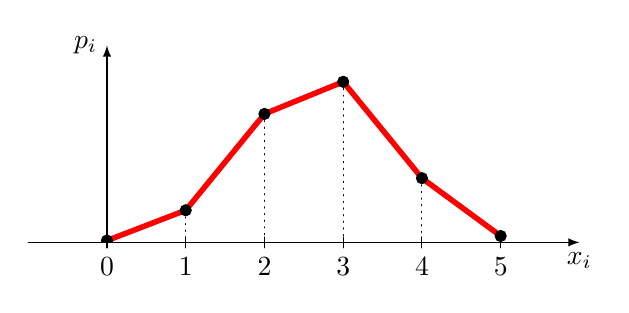
\begin{tikzpicture}[
	x=1cm,
	y=5cm,
	line join=round,
	line cap=round,
	>=latex,
	]
\draw[->] (-1,0) -- (6,0) node[below] {$x_i$};
\draw[->] (0,0) -- (0,.5) node[left] {$p_i$};
\coordinate (a) at (0,2/429);
\coordinate (b) at (1,35/429);
\coordinate (c) at (2,140/429);
\coordinate (d) at (3,175/429);
\coordinate (e) at (4,70/429);
\coordinate (f) at (5,7/429);
\draw[line width=2pt, red] (a) -- (b) -- (c) -- (d) -- (e) -- (f);
\foreach \x in {0, 1, 2, 3, 4, 5}
	\draw[xshift=\x cm] (0,2pt) -- (0,-2pt) node[below] {$\x$};
\clip (-.2,0) rectangle (6,.5);
\foreach \p in {a, b, c, d, e, f}
	{
	\draw[fill] (\p) circle (2pt);
	\draw[dotted] (\p) -- +(0,-1);
	}
\end{tikzpicture}
}
\end{figure}

\par  б) функция распределения и ее график:
\begin{figure}[h!]
\parbox{.5\tablew}{
$$F(x) = \begin{cases}
0, 			&x \leqslant 0, \\
2 / 429, 	&0 < x \leqslant 1, \\
37 / 429, 	&1 < x \leqslant 2, \\
177 / 429, 	&2 < x \leqslant 3, \\
352 / 429, 	&3 < x \leqslant 4, \\
422 / 429, 	&4 < x \leqslant 5, \\
1,			&x > 5.
\end{cases}$$
}
\parbox{.5\tablew}{
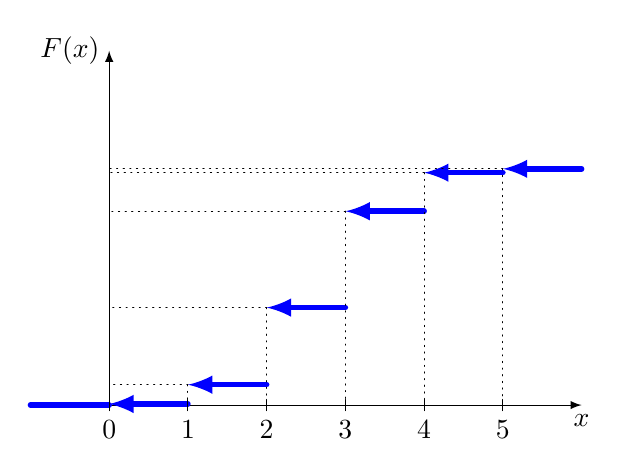
\begin{tikzpicture}[
	x=1cm,
	y=3cm,
	line join=round,
	line cap=round,
	>=latex,
	]
\draw[->] (-1,0) -- (6,0) node[below] {$x$};
\draw[->] (0,-.02) -- (0,1.5) node[left] {$F(x)$};
\draw[line width=2pt, blue] (-1,0) -- (0,0);
\coordinate (a) at (0,2/429);
\coordinate (b) at (1,37/429);
\coordinate (c) at (2,177/429);
\coordinate (d) at (3,352/429);
\coordinate (e) at (4,422/429);
\coordinate (f) at (5,1);
\foreach \p in {a, b, c, d, e, f}
	\draw[<-, line width=2pt, blue] (\p) -- +(1,0);
\foreach \x in {0, 1, 2, 3, 4, 5}
	\draw[xshift=\x cm] (0,2pt) -- (0,-2pt) node[below] {$\x$};
\clip (0,0) rectangle (6,1);
\foreach \p in {a, b, c, d, e, f}
	{
	\draw[dotted] (\p) -- +(0,-1);
	\draw[dotted] (\p) -- +(-6,0);
	}
\end{tikzpicture}
}
\end{figure}

\par  в) математическое ожидание $M(X) = \frac{35}{13}$.

\par  г) дисперсия $D(X) = \frac{140}{169}$; 
среднее квадратическое отклонение $\sigma = \frac{2\sqrt{35}}{13}$. 

\end{zkrPlain}

\newpage


\begin{zkrPlain}{25} Найти математическое ожидание $M(X)$, дисперсию $D(X)$ и вероятность $P(X>1/2)$ непрерывной случайной величины с плотностью вероятностей $f(x)$, заданной графически\footnote{график может быть составлен лишь из участков прямых и парабол.}. 
\begin{figure}[h!]\centering\small
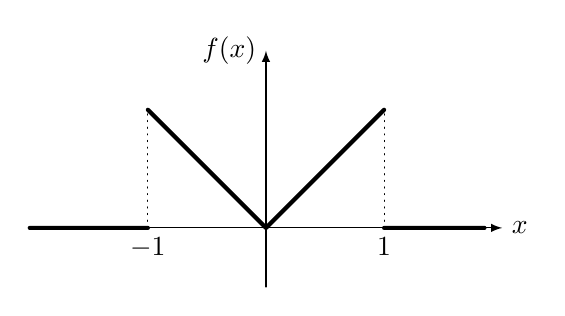
\begin{tikzpicture}[
		x = 1.5cm,
		y = 1.5cm,
		line join = round,
		line cap = round,
		> = latex,
		]
\draw[->]	(-2,0) -- (2,0)	node[right]	{$x$};
\draw[->]	(0,-.5) --  (0,1.5)	node[left]	{$f(x)$};
\draw[line width=1.5pt]		(-1,1) -- (0,0) --  (1,1)
				(-2,0) -- (-1,0)
				(1,0) -- (1.85,0);
\draw[dotted]		(-1,0) node[below] {$-1$} -- (-1,1);
\draw[dotted]		(1,0)  node[below] {$\vphantom{-}1$} -- (1,1);
\end{tikzpicture}
\end{figure}

а) математическое ожидание $M(X) = 0$.

б) дисперсия $D(X) = \frac{1}{2}$.

в) вероятность $P(X>1/2) = \frac{3}{9}$.

\end{zkrPlain}

\vfil

\begin{zkrPlain}{25} Вес рыб, обитающих в водоеме, подчиняется нормальному закону с параметром $a = 375$ г. Вероятность того, что вес пойманной рыбы меньше $400$ г, равна $0{,}8413$. 

\zzz вероятность того, что вес выловленной наудачу рыбы попадет в промежуток от $300$ г до $425$ г: 
$$P(300<X<425) = 0{,}9759. $$

\zzz квантиль уровня $0{,}7$ 
$$x_{0{,}7} = 388{,}11.$$

\end{zkrPlain}

\vfil


\begin{zkrPlain}{25} В осветительную сеть параллельно включено 20 ламп. Вероятность того, что за время $T$ лампа будет включена, равна $0{,}8$. Пользуясь неравенством Чебышева, оценить вероятность того, что абсолютная величина разности между числом включенных ламп и средним числом (математическим ожиданием) включенных ламп за время $T$ окажется: 

а) меньше трех: $$P\left(|X-M(X)|<3\right) \geqslant 0{,}644.$$

б) не меньше трех: $$P\left(|X-M(X)|\geqslant 3\right) \leqslant 0{,}356.$$


\end{zkrPlain}

\end{document}